\documentclass{article}

\usepackage{fancyhdr}
\usepackage{extramarks}
\usepackage{amsmath}
\usepackage{minted}
\usepackage{amsthm}
\usepackage{amsfonts}
\usepackage{tikz}
\usepackage[plain]{algorithm}
\usepackage{algpseudocode}
\usepackage{graphicx}
\usepackage{caption}
\usepackage{subcaption}

\usetikzlibrary{automata,positioning}
\usepackage{fullpage,enumitem,amsmath,amssymb,graphicx}

%
% Basic Document Settings
%

\topmargin=-0.75in
\textwidth=6.5in
\textheight=9.0in
\headsep=0.20in
\headheight = 12pt
\linespread{1.1}

\pagestyle{fancy}
\chead{\hmwkClass\ (\hmwkClassInstructor): \hmwkTitle}
\rhead{\firstxmark}
\lfoot{\lastxmark}
\cfoot{\thepage}

\renewcommand\headrulewidth{0.55pt}
\renewcommand\footrulewidth{0.55pt}

\setlength\parindent{0pt}


\setcounter{secnumdepth}{0}

%
% Homework Problem Environment
%
% This environment takes an optional argument. When given, it will adjust the
% problem counter. This is useful for when the problems given for your
% assignment aren't sequential. See the last 3 problems of this template for an
% example.

%
% Homework Details
%   - Title
%   - Due date
%   - Class
%   - Section/Time
%   - Instructor
%   - Author
%

\newcommand{\hmwkTitle}{Homework\ \#7}
\newcommand{\hmwkDueDate}{November 07, 2021}
\newcommand{\hmwkClassCode}{COT 5615}
\newcommand{\hmwkClass}{Math for Intelligent Systems}
\newcommand{\hmwkClassYear}{Fall 2021}
\newcommand{\hmwkClassInstructor}{Professor Kejun Huang}
\newcommand{\hmwkAuthorName}{\textit{Vyom Pathak}}
\newcommand{\hmwkUFID}{96703101}

%
%
%
% Various Helper Commands
%

% Useful for algorithms
\newcommand{\alg}[1]{\textsc{\bfseries \footnotesize #1}}

% For derivatives
\newcommand{\deriv}[1]{\frac{\mathrm{d}}{\mathrm{d}x} (#1)}

% For partial derivatives
\newcommand{\pderiv}[2]{\frac{\partial}{\partial #1} (#2)}

% Integral dx
\newcommand{\dx}{\mathrm{d}x}

% Alias for the Solution section header
\newcommand{\solution}{\textbf{\large Solution}}

% Probability commands: Expectation, Variance, Covariance, Bias
\newcommand{\E}{\mathrm{E}}
\newcommand{\Var}{\mathrm{Var}}
\newcommand{\Cov}{\mathrm{Cov}}
\newcommand{\Bias}{\mathrm{Bias}}

% norm bars
\newcommand{\norm}[1]{\left\lVert#1\right\rVert}

\begin{document}

\begin{center}
{\Large \hmwkClassCode\ \hmwkClass\ \hmwkClassYear\ \hmwkTitle}

\begin{tabular}{rl}
UFID: & \hmwkUFID \\
Name: & \hmwkAuthorName \\
Instructor: & \hmwkClassInstructor \\
Due Date: & \hmwkDueDate \\ 
% Collaborators: & [list all the people you worked with]
\end{tabular}
\end{center}

\section*{Problem 10.16}
\subsection*{Covariance matrix}
\subsubsection*{Solution}
\begin{enumerate}[label=(\alph*)]
    \item $\mu=\frac{A^T\cdot1}{n}$
    \item As it is the de-meaned value, $\widetilde{A} = A-1\mu^T$.
    Here, $\widetilde{a_i} = a_i-\mu_i1$, thus $\widetilde{A}$ can be shown as follows:
    \begin{align*}
        \widetilde{A} & = (a_1; a_2; \ldots; a_k) - (\mu_11; \mu_21; \ldots; \mu_k1)\\
        & = (a_1; a_2; \ldots; a_k) - 1(\mu_1; \mu_2; \ldots; \mu_k)\\
        & = A-1\mu^T
    \end{align*}
    \item The diagonal entries $\sum_{ii}$ are given as follows:
    \begin{align*}
        \sum_{ii} & = \frac{(\widetilde{A}^T\widetilde{A})_{ii}}{N}\\
        & = \frac{\widetilde{a_i}\widetilde{a_i}^T}{N}\\
        & = \frac{\norm{\widetilde{a_i}}^2}{N}\\
        & = std(a_i)^2\ [\because standard\ deviation\ std(a_i)=\frac{\norm{\widetilde{a_i}}}{\sqrt{N}}]
    \end{align*}
    Now, the off-diagonal entries of $\sum_ij$ is zero where $\widetilde{a}_i=0$ and $\widetilde{a}_j=0$. For other values, it is calculated as follows:
    \begin{align*}
        \sum_{ij} & =  \frac{(\widetilde{A}^T\widetilde{A})_{ii}}{N}\\
        & = \frac{\widetilde{a_i}\widetilde{a_j}^T}{N}\\
        & = \rho_{ij}std(a_i)std(a_j)\ \left[\because \rho_{ij} = \frac{\widetilde{a_i}\widetilde{a_j}^T}{N\cdot std(a_i)std(a_j)}\right]
    \end{align*}
    \item $Z = (A-1\mu^T)diag(\frac{1}{std(a_1)};\frac{1}{std(a_2)};\ldots\frac{1}{std(a_k)})$. Here, $z_i = \frac{\widetilde{a_i}}{std(a_i)}$ are the standardized vectors. Thus the above solution can be derived as follows:
    \begin{align*}
        Z & = \widetilde{A}\cdot diag(\frac{1}{std(a_1)};\frac{1}{std(a_2)};\ldots\frac{1}{std(a_k)})\\
        & = (A-1\mu^T)\cdot diag(\frac{1}{std(a_1)};\frac{1}{std(a_2)};\ldots\frac{1}{std(a_k)})
    \end{align*}
    
\end{enumerate}
\section*{Problem A14.3}
\subsection*{Iris classification}
\subsubsection*{Solution}
The following code is used to find the least square solution for each class of the iris data and also the multi-class classification model is built by using the single regression model together :
    \begin{minted}[
frame=lines,
framesep=2mm,
baselinestretch=1.2,
fontsize=\footnotesize,
linenos
]{julia}
    # Using this imports for all the solutions.
    using Statistics
    using LinearAlgebra
    using Plots
    using MLJ
    plotly()
    
    include("iris_flower_data.jl")
    include("iris_multiclass_helpers.jl")
    # function to get and format dataset 
    function get_iris_data()
        Random.seed!(5)
        # Formatting dataset (must Pkg.add("RDatasets"))
        iris = dataset("datasets", "iris")
        data = Matrix(iris)
        X = transpose(1.0*data[:, 1:4]);
        perm = randperm(150);
        X = X[:, perm]; 
        y = [ones(50); 2*ones(50); 3*ones(50)];
        y = y[perm];
        return (X, y)
    end
    
    D = get_iris_data();
    X_train = D[1][1:4,1:100]';
    Y_train = D[2][1:100];
    
    Theta1 = X_train\((2*(Y_train.==1)).-1); 
    Theta2 = X_train\((2*(Y_train.==2)).-1);
    Theta3 = X_train\((2*(Y_train.==3)).-1);
    
    X_test = D[1][1:4,101:150]';
    Y_test = D[2][101:150];
    
    #a
    #Train errors
    display(mean((X_train*Theta1.>0) .!=(Y_train.==1)));
    display(mean((X_train*Theta2.>0) .!=(Y_train.==2)));
    display(mean((X_train*Theta3.>0) .!=(Y_train.==3)));
    
    #Test errors
    display(mean((X_test*Theta1.>0) .!=(Y_test.==1)));
    display(mean((X_test*Theta2.>0) .!=(Y_test.==2)));
    display(mean((X_test*Theta3.>0) .!=(Y_test.==3)));
    
    #b 
    #confusion_matrix for train and test
    display(confusion_matrix(argmax_by_row((X_train*[Theta1 Theta2 Theta3])), Y_train));
    display(confusion_matrix(argmax_by_row((X_test*[Theta1 Theta2 Theta3])), Y_test));    

    \end{minted}
    \begin{enumerate}[label=(\alph*)]
        \item Class 1 error rate for train data: 0.0\\
Class 2 error rate for train data: 0.28\\
Class 3 error rate for train data: 0.36\\\\
Class 1 error rate for test data: 0.0\\
Class 2 error rate for test data: 0.24\\
Class 3 error rate for test data: 0.28\\
        \item The confusion matrix for training data (upper) and testing data (lower) is shown in the figure~\ref{fig:conf_matrix}:
        \begin{figure}[h]
            \centering
            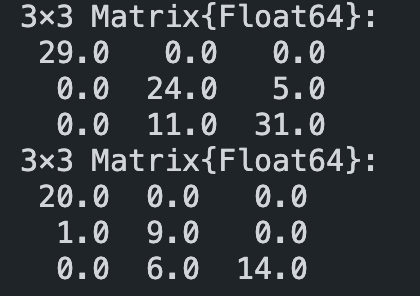
\includegraphics{Train_Test_Conf.png}
            \caption{Confusion Matrix for training data (upper) and testing data for iris multi-class classification}
            \label{fig:conf_matrix}
        \end{figure}
    \end{enumerate}
\section*{Problem A15.2}
\subsection*{Least squares classification with regularization}
\subsubsection*{Solution}
    \begin{minted}[
frame=lines,
framesep=2mm,
baselinestretch=1.2,
fontsize=\footnotesize,
linenos
]{julia}
    include("lsq_classifier_data.jl")
    
    #a
    A = [ones(size(X)[2]) X'];
    
    Theta = A\y;
    v = Theta[1,:]
    beta = Theta[2:51];
    println("Beta and v (slope) values are : ", beta, v);
    
    y_hat = X' * beta .+ v;
    test_y_hat = X_test' * beta .+ v;
    println("The error rate on training data is ",(sum(((y_hat).>0) .!=(y.==1)) + sum(((y_hat).<0) .!=(y.==-1)))
    /size(y)[1]/2);
    println("The error rate on testing data is ",(sum(((test_y_hat).>0) .!=(y_test.==1)) + sum(((test_y_hat).<0) .!=
    (y_test.==-1)))/size(y_test)[1]/2);
    
    #b
    regularization_factor =  10 .^ range(-1,4,length = 100);
    test_values = []
    train_values = []
    logvalues = []
    for i in regularization_factor
        Theta = inv(transpose(A)*A + i*Matrix{Float64}(I,51,51)) * transpose(A) * y;
        v = Theta[1,:]
        beta = Theta[2:51];
        y_hat = X' * beta .+ v;
        test_y_hat = X_test' * beta .+ v;
        append!(train_values,(sum(((y_hat).>0) .!=(y.==1)) + sum(((y_hat).<0) .!=(y.==-1)))/size(y)[1]/2);
        append!(test_values,(sum(((test_y_hat).>0) .!=(y_test.==1)) + sum(((test_y_hat).<0) .!=
        (y_test.==-1)))/size(y_test)[1]/2);
        append!(logvalues,log10(i));
    end
    
    plot(logvalues, xlabel = "Log Scaled Lambdas", ylabel = "RMS Error", train_values, label = "Train Data")
    plot(logvalues, xlabel = "Log Scaled Lambdas", ylabel = "RMS Error", test_values, label = "Test Data")
    println("Regularization value at minimum loss value for train data is ", regularization_factor[findmin(train_values)[2]]);
    \end{minted}
    \begin{enumerate}
        \item The error rate is as follows:\\
        The error rate on training data is 0.2\\
        The error rate on testing data is 0.28\\
        The beta and v (slope) values follows:\\
        ( -0.013368564887362284, 0.043914619202142506, -0.029703277493729204, 0.0441447412881381, -0.07058131397505582, 0.007607031569404489, 0.14833182533722705, 0.02852393154963966, 0.019812521586858763, -0.12070927744292764, 0.013784598389068807, 0.07897384306339864, -0.016767001698145247, 0.03105477750315689, 0.006356245285928464, -0.09111311295164341, 0.0046968705247653515, -0.03371811652421457, 0.014237165383124077, -0.1715950849684703, 0.05418932576076964, -0.06405036863460692, -0.0446363886361793, 0.060640599059827535, 0.022398446473252752, 0.01634655578292057, 0.028027646705782807, 0.046686592731404526, -0.13392652651935205, -0.09059400055804874, -0.0879007600259256, 0.010548532354429147, -0.03467602240482772, -0.06877162458039814, -0.05169326750991447, 0.13547906032991633, 0.07853780188316374, 0.11922412326678362, 0.026479714104205146, -0.053715275373795564, -0.1858378466312867, -0.06173600519777898, -0.05090661312828648, -0.0026805843235918987, 0.007823258649938056, -0.02354617634571561, 0.13831311716195221, 0.02153524018622994, -0.0036408708130813467, -0.10621012236954906 ) ( 0.3679341344425215 )
        \item Regularization value at minimum loss value for test data is 23.644894126454073. The figure~\ref{fig:train_test_reg}
        \begin{figure}[htp]
            \centering
            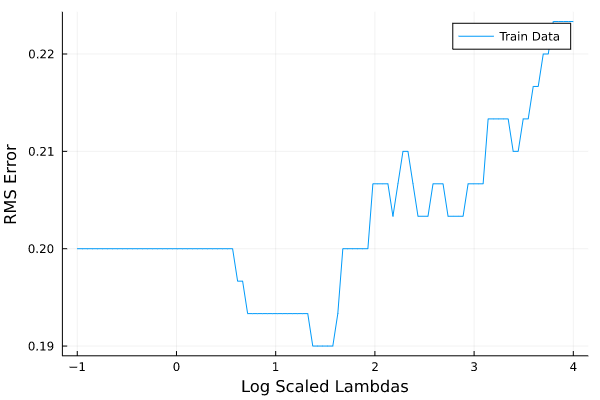
\includegraphics[width=.50\textwidth]{15.2.b.1.png}\hfill
            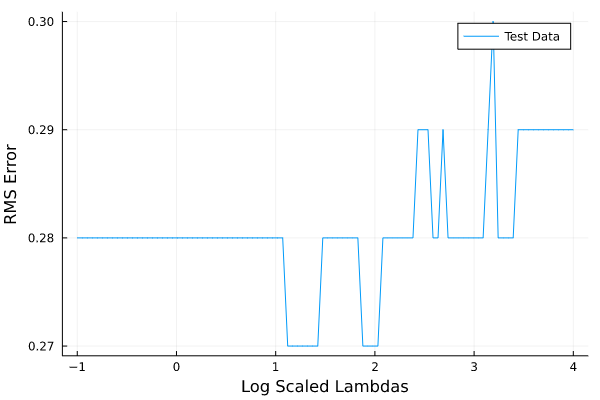
\includegraphics[width=.50\textwidth]{15.2.b.2.png}\hfill
            \caption{Train and test regularization loss versus the lambda value}
            \label{fig:train_test_reg}
        \end{figure}
    \end{enumerate}
    
\section*{Problem A15.3}
\subsection*{Estimating the elasticity matrix}
\subsubsection*{Solution}
Give the price, demand data, it can be easily transformed into a least square problem, where $\delta^d \approx \hat{E}\delta^p$ is the modeling equation. Here, first we find the delta values using the given formula. After, that we estimate elastic matrix by performing least square regression for each price value, and thus get a NXN elastic matrix. We the test this elastic matrix by using it to find change in demand for unseen data and check it's efficacy by calculating RMSE value. We perform a 80-20 split in 75 items i.e. 60 items for training and 15 items for testing. We find that, the RMSE for test and train unseen data is given as 0.208629686471379 and 0.26213391380879586. This indicates that the elastic matrix is performing welll in terms of finding change in demand for new (unseen) change in prices and thus it is not showing any amount of overfitting.
\begin{minted}[
frame=lines,
framesep=2mm,
baselinestretch=1.2,
fontsize=\footnotesize,
linenos
]{julia}
    include("price_elasticity.jl")
    
    delta_p = zeros(5,75)
    delta_d = zeros(5,75)
    for product in 1:5
      delta_p[product,:] = (Prices[product,:].- p_nom[product])./p_nom[product];
      delta_d[product,:] = (Demands[product,:].- d_nom[product])./d_nom[product]; 
    end
    
    delta_p_train = delta_p[1:5,1:60];
    delta_p_test = delta_p[1:5,61:75];
    delta_d_train = delta_d[1:5,1:60];
    delta_d_test = delta_d[1:5,61:75];
    
    E_cap = zeros(5,5)
    
    for product in 1:5
      E_cap[product,:] = (delta_d[product,:]\transpose(delta_p))
    end
    
    display(E_cap);
    display(E);
    
    delta_d_hat = E_cap * delta_p_test
    println("The RMS Error for the training change in demand is ", rms(E_cap * delta_p_train, delta_d_train));
    println("The RMS Error for the unseen change in demand is ", rms(delta_d_hat, delta_d_test));
\end{minted}
\end{document}
